\documentclass{article}
\usepackage{geometry}
\usepackage{blindtext}
\usepackage[T1]{fontenc}
\usepackage[utf8]{inputenc}

\usepackage{makecell}
\usepackage{amsfonts}
\usepackage{longtable}
\usepackage{amsmath}
\usepackage{amssymb}
\usepackage{amsthm}
\usepackage{systeme}
\usepackage{graphicx}
\graphicspath{ {./images/} }


\setlength\parindent{24pt}

\title{Singular Value Decomposition}
\author{Vincent Mollicone, Chris Lee, and Helen Chen}
\date{\today}

\geometry{margin=1in, top=0.5in}

\begin{document}

\maketitle

\section{Introduction}
\subsection{What is Singular Value Decomposition?}


\section{Theories}
\subsection{Motivation}
The singular value decomposition, often refer to as SVD, is the best factorization of any matrix:
$$A = U \Sigma V^T$$
where $U,T$ are orthonormal and $\Sigma$ is diagonal.

Recall from MATH 308 that if we have a symmetric matrix $A$, then we can diagonalize it with the form $A=PDP^{-1}$ where $P$ is the orthonormal eigenvectors and $D$ is diagonal. This is just a special case of the SVD, that $P = U = V$.

The essence of SVD is very simple. That is, having a linear transformation $A$ from $\mathbb{R}$ to $\mathbb{R}$ (for $\mathbb{C}$ to $\mathbb{C}$ if $A$ is complex), we want to find an orthonormal basis ($\vec{v}_i$'s) in the domain such that the image of this basis are still orthogonal (a scaler multiple of $\vec{u}_i$ where $\vec{u}_i$'s orthogonal) after the transformation $A$. In linear algebra language, this means 
\begin{align*}
AV =A \begin{pmatrix} \vec{v}_1 & \vec{v}_2 & \cdots & \vec{v}_n  \\ \downarrow & \downarrow & &\downarrow \end{pmatrix} &= \begin{pmatrix} \sigma_1 \vec{u}_1 & \sigma_2 \vec{u}_2 & \cdots &\sigma_n \vec{u}_n  \\ \downarrow & \downarrow & &\downarrow \end{pmatrix} \\
&= \begin{pmatrix} \vec{u}_1 & \vec{u}_2 & \cdots & \vec{u}_n  \\ \downarrow & \downarrow & &\downarrow \end{pmatrix} \begin{pmatrix} \sigma_1 & 0 & \cdots & 0 \\ 0& \sigma_2 & \cdots & 0 \\ \vdots & \vdots & \ddots & \sigma_n \end{pmatrix} \\
&= U \Sigma
\end{align*}
where $\vec{v}_1, \vec{v}_2, \cdots, \vec{v}_n$ are orthonormal to each other (hence $V$ orthonormal), $\vec{u}_1, \vec{u}_2, \cdots, \vec{u}_n$ are orthonormal orthonormal to each other (hence $U$ orthonormal), and $\Sigma$ is diagonal.

Since $V$ is orthogonal, $V^{-1} = V^T$, hence after rearranging we have
\begin{align*}
AV &= U \Sigma \\
AV V^{-1} &= U \Sigma V^{-1} \\
A &= U\Sigma V^T
\end{align*}
then we get the decomposition form we had for $A$.

\subsection{How to calculate SVD}
For a given $A$, in order to find $U, \Sigma, V$ such that $A = U \Sigma V^T$ (where $U,V$ orthonormal and $\Sigma$ diagonal), there are a few preliminary results we need to prove.
\bigskip

\textit{\textbf{Def:}} \textit{A real $n \times n$ matrix $A$ is symmetric positive definite if it is symmetric (i.e. $A=A^T$) and 
$$ x^T A x > 0 \text{ for all nonzero vectors }x$$
If $A$ is symmetric positive semi-definite, then the strict grater sign changes to greater than or equal to.}
\bigskip

There are some nice theorems we can prove about symmetric positive definite matrix, which are essential for our calculation of SVD.
\bigskip

\textit{\textbf{Theorem 1:}} \textit{Let $A$ be a positive definite real matrix, then the eigenvalues of $A$ are positive.}

\begin{proof}
Let $\lambda$ be an eigenvalue of $A$ and $x$ be the corresponding eigenvector. Then 
\begin{align*}
Ax &=\lambda x \\
x^T A x &= \lambda x^Tx  = \lambda || x ||^2 
\end{align*}
Note that $x^T x$ is just a normal inner product of $x$ with itself, that is, the sum of each component square.
  
Since A is positive definite, $x^T A x =\lambda ||x||^2> 0$. Because the norm $||x||^2 $ is the square of a non-zero number ($x$ is an eigenvector, so must be non-zero), it must be positive. Hence $$\lambda > \frac{0}{||x||^2} = 0$$
\end{proof}

Note that the above proof translates to a symmetric positive semi-definite matrix, in this case, the eigenvalues are non-negative ($\lambda \ge 0$).
\bigskip

\textit{\textbf{Theorem 2:}} \textit{Let $A$ be any matrix, then $AA^T$ and $A^TA$ are symmetric positive semi-definite.}

\begin{proof}
First, we will show that $AA^T$ is symmetric.

Write $$A = \begin{pmatrix} \vec{a}_1  & \rightarrow \\
\vec{a}_2 & \rightarrow \\ \vdots \\ \vec{a}_n & \rightarrow\end{pmatrix} $$
then $$A^T = \begin{pmatrix} \vec{a}_{1} & \vec{a}_{2}  & \cdots  &\vec{a}_n\\
\downarrow &\downarrow  &  & \downarrow \end{pmatrix} $$
Taking the product, we have
$$ A A^T = \begin{pmatrix} \vec{a}_1  & \rightarrow \\
\vec{a}_2 & \rightarrow \\ \vdots \\ \vec{a}_n & \rightarrow\end{pmatrix}  \begin{pmatrix} \vec{a}_{1} & \vec{a}_{2}  & \cdots  &\vec{a}_n\\
\downarrow &\downarrow  &  & \downarrow \end{pmatrix} = \begin{pmatrix} \vec{a}_1 \cdot \vec{a}_1 & \vec{a}_1 \cdot \vec{a}_2  & \cdots & \vec{a}_1 \cdot \vec{a}_n\\ \vec{a}_2 \cdot \vec{a}_1 & \vec{a}_2 \cdot \vec{a}_2 & \cdots &\vec{a}_2 \cdot \vec{a}_n \\
\vdots& \vdots & \ddots & \vdots \\
\vec{a}_n \cdot \vec{a}_1 & \vec{a}_n \cdot \vec{a}_2 & \cdots & \vec{a} _n \cdot \vec{a}_n \end{pmatrix} 
$$
Note that here $a_i \cdot a_j = a_{i1}a_{j1} + a_{i2}a_{j2} + \cdots + a_{in}a_{jn}$, so $a_i \cdot a_j = a_j \cdot a_i$, hence the above matrix is symmetric.

Now we will show that $AA^T$ is positive semi-definite. Using the formula for the transpose of a product, we can write
$$x^T AA^T x = (A^Tx)^T (A^Tx) $$

Notice that $(A^Tx)$ is just a column vector, let's call it $y$. Then we have $x^T AA^T x = y^T y = ||y||^2 \ge 0$. This shows $AA^T$ is positive semi-definite. 

Let $A \rightarrow A^T$, then the same prove will show that $A^TA$ is also positive semi-definite.
\end{proof}
\bigskip

Another theorem we will need is a theorem we have used from MATH 308. That is, 
\bigskip

\textit{\textbf{Theorem 3:}} \textit{Let $A$ be a $n \times n $ symmetric matrix, then we can write $A= P D P^{-1}$ where $P$ is orthonormal and have eigenvectors of $A$ as its columns, and $D$ is diagonal with eigenvalues of $A$ as diagonal entries.}

\begin{proof}
(see textbook, theorem 6.19 and 6.20)
\end{proof}
\bigskip 

Now, equipped with these theorems, we can proceed to find a formula for $U, \Sigma, V$. 
\bigskip

Given $A= U \Sigma V^T$ (where $U,V$ orthonormal and $\Sigma$ diagonal), to first find $V$ and $\Sigma$, we write the following 
$$A^TA = ( U \Sigma V^T)^T ( U \Sigma V^T) = V \Sigma^T U^T U \Sigma V^T$$
It is easy to see that if $D$ is diagonal then $D^T = D$ and $D^n$ can be calculated by taking each entry to the $n$th power. Moreover, in lecture 25, we learned that if a matrix $P$ is orthonormal, then $P^{-1} = P^T$. Plugging in these relations, we have 
$$A^TA =V \Sigma^T U^T U \Sigma V^T = V \Sigma^T U^{-1} U \Sigma V^T =V \Sigma^T  \Sigma V^T = V \Sigma^2 V^{-1}$$
Since $A^TA$ is symmetric positive semi-definite by theorem 2 (in particular it is symmetric), this is just the form of diagonalization we are familiar with from 308 (theorem 3), that is, $$V = \begin{pmatrix} \vec{v}_{\lambda_1} & \vec{v}_{\lambda_2} & \cdots & \vec{v}_{\lambda_m} \end{pmatrix}, \; \Sigma^2 = \begin{pmatrix} \sigma^2_1 & 0&  \cdots & 0 \\ 0& \sigma^2_2 &\cdots & 0 \\ \vdots & \vdots & \ddots &0 \\
0 &0& \cdots & \sigma^2_m  \end{pmatrix}$$ 
where $\sigma^2_i$ are eigenvalues of $A^TA$ and $\vec{v}_{\lambda_i}$ are the corresponding normalized orthogonal eigenvectors. Notice that since $A^TA$ is positive semi-definite, the eigenvalues are non-negative (theorem 1) and so $\sigma_i \in \mathbb{R}$. So in the case where $A$ is real, we won't have $A$ mapping to a complex vector space. 
\bigskip

Similarly, we can obtain $U$ by writing,
$$AA^T = (U \Sigma V^T)(U \Sigma V^T)^T = U \Sigma V^T V \Sigma^TU^T = U \Sigma  \Sigma^TU^T = U  \Sigma^2U^{-1}$$
Then 
$$U = \begin{pmatrix} \vec{u}_{\lambda_1} & \vec{u}_{\lambda_2} & \cdots & \vec{u}_{\lambda_m} \end{pmatrix}$$ 
where $\vec{u}_{\lambda_i}$ are normalized orthogonal eigenvectors corresponding to the same set of $\Sigma^2$. One thing we have to be careful is that the order of $\vec{u}_{\lambda_i}$'s matters. They must be in the order conformed with the order of eigenvalues in $\Sigma^2$.

\subsection{Examples}

\newpage
\section{Application - Principal Component Analysis}
\subsection{What Is Principal Component Analysis?}
Take a look at the following table of food consumption.

\begin{center}
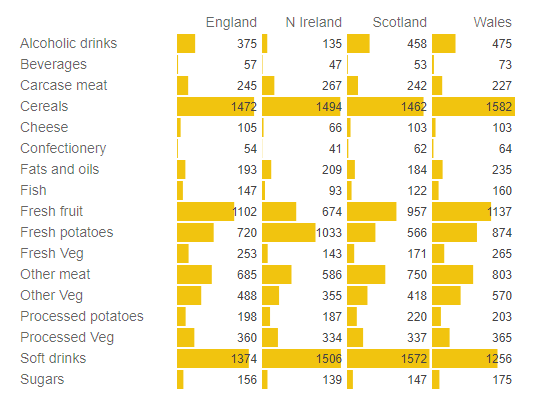
\includegraphics[width=12cm]{(17)}
\end{center}


Suppose you wanted to see if one of these countries consumes a diet different that the others. How would you do that? At first glance they all seem very similar. You might notice some interesting variation among certain food types, but the overall variation is certainly not obvious.
\bigskip

We can use a process called principal component analysis (PCA) to help us out. PCA is a factorization of used for reducing the dimensions of a multivariate data set. Furthermore, when it reduces the dimensions, it does so by removing dimension with the least variability, perfect for this situation.
\bigskip

By applying PCA, we can reduce the 17 variables to only two and create a nice, easy to read, graph.

\begin{center}
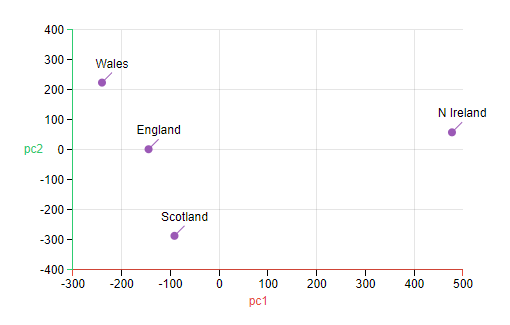
\includegraphics[width=12cm]{(18).png}
\end{center}

From here it is obvious that Northern Ireland's diet is different than the other countries. This makes sense because Northern Ireland is the only of the four countries not on the Island of Great Britain!

\subsection{How to do a Principle Component Analysis}
PCA is done using all the framework we have built up studying the SVD. In fact, PCA is simply a statistical interpretation of the SVD. It has slightly different language as the the literature for PCA uses different conventions than the SVD literature but the concepts are analogous. Let's walk through the steps to compute do the principal component analysis shown above.
\bigskip

\begin{enumerate}
\item Setting Up: First, we need to set up a matrix that contains our data. This can be easily done by simply putting the number in the spot in the matrix where it appears in the table. If we call this matrix $A$, which would be a matrix in $\mathbb{R}^{17\times 4}$, then $A_{1,1}=375$ which is the Alcoholic drinks consumed in England. By convention, the matrices for PCA have experiments (in our example we have four: England, N Ireland, Scotland, and Wales) as rows. Ours are columns so we will simply use the transpose.

\item Mean-Centering: The second set up step is called mean centering. Our data has an underlying distribution. For reasons having to do with the statistics of the PCA we want the mean of each row to be zero. This centers the underlying distribution of the data around 0. To do this we must compute the mean of each row then subtract it. This looks like:
$$~$$
Let $A$ be our data matrix. First we compute the mean for each row,
$$\bar{a}=\frac{1}{n}\sum_{j=1}^n a_j$$
$$\bar{A}=\begin{bmatrix}1\\1\\\vdots\\1\end{bmatrix}\left[~\,\bar{a}\,~\right]$$

Subtract the mean.
$$B=A-\bar{A}$$

\item The covariance matrix: Now we get what is called a covriance matrix for the rows of $B$. We will call this matrix $C$ and we get it by performing
$$C=B^\top B$$

\item The eigen-decomposition: This means we need to find the eigenvalues and eigenvectors of $C$. In particular we want to find $v_1^\top B^\top B v_1$ where $v_1$ is the largest eigenvector of of $C$ then do the same for $v_2$, $v_3$, and so on just like in the SVD. The result is that we have $$CV=VD$$ where $V$ is the eigenvectors for $C$ and $D$ is the eigenvalues.

\item Principal Components: We define the matrix of principle components of $B$ as $T$. We can equivalently define $T$ as the matrix such that,
$$T=BV$$
Recall that $B$ is our data matrix with the mean of each row subtracted off and $V$ is the eigenvectors of $C$. In PCA language, $V$ is also called the "loadings" of the principal components. The loadings are the directions of maximal variance, similar to the singular values of the SVD. In fact, in the language of the SVD, if we let $B=U\Sigma V^\top$, the SVD factorization, then we can say that,
$$T=BV=U\Sigma$$
What this means is that we can also find the PCA simply using the SVD!

\item Interpreting the Principle Components: We have the principal components, now what? What do these mean? The eigenvalues of $C$, found in step 4 (also the singular values of the SVD of $B$) represents the amount of variance captured by the particular loading $V$. In many cases most of the variance will be captured in the first few principal components. It follows from this that if we want to reduce the dimensions, say to dim $k$, of our data matrix we can simply take the matrix composed of the first $k$ principal components. We can then explicitly compute the amount of variance retained in our reduced matrix by taking the sum of the eigenvalues (singular values of SVD) of the principal components of the reduced matrix and dividing them by the total. For a rank $n$ matrix and a rank $k$ reduced matrix this looks like,

$$\text{Var}(B)=\frac{\sum_{j=1}^{k}\lambda_j}{\sum_{j=1}^{n}\lambda_j}$$

Or equivalently in the language of the SVD,

$$\text{Var}(B)=\frac{\sum_{j=1}^{k}\sigma^2_j}{\sum_{j=1}^{n}\sigma^2_j}$$


Going back to the example in the introduction we can see that we used the first two principal components to create a nice 2 dimensional graph that was able to answer our question. Now that we got the idea of what PCA we will do a simple example to get a feel for how the computations look.
\end{enumerate}

\subsection{Example problem}
Suppose we have math scores and history scores of six students. Our data points are of the form $(x_i,y_i)$ where $x_i$ denotes the math score of student $i$ and $y_i$ denotes the
history score of student $i$. After setting up and centering the data (step 1 and 2) we get,

$$\begin{bmatrix}
3& -4& 7& 1& -4& -3\\
7& -6& 8& -1& -1& -7
\end{bmatrix}$$

\noindent Compute the principal components.

\bigskip

\textbf{Solution:} We can do this easily using the SVD! First, observe that the first two steps are done for us. Let us call the matrix above $B$ to remain consistent. Thus,

$$B=\begin{bmatrix}
3&-4&7&1&-4&-3\\
7&-6&8&-1&-1&-7
\end{bmatrix}$$

Recall that we can get the principal components of $B$ directly by computing the SVD. This is what we will do. The SVD of $B$ is,

$$B=U\Sigma V^\top$$

Computing this we have,

\begin{align}
B&=U\Sigma V^\top\\
&=\begin{bmatrix}
-0.560&-0.828\\
-0.828&0.560\end{bmatrix}
\begin{bmatrix}
16.870&0\\
0&3.920
\end{bmatrix}
\begin{bmatrix}-0.443&0.427&-0.625&0.015&0.182&0.443\\
0.367&-0.013&-0.334&-0.354&0.701&-0.367\end{bmatrix}
\end{align}

(If you need a refresher about how to compute the SVD see the SVD notes)

We know from step five,

\begin{align}
T&=U\Sigma\\
&=\begin{bmatrix}
-0.560&-0.828\\
-0.828&0.560\end{bmatrix}
\begin{bmatrix}
16.870&0\\
0&3.920
\end{bmatrix}
\end{align}

Thus we have principal components
$$u_1=\begin{pmatrix}
-0.560\\
-0.828\end{pmatrix},u_2=\begin{pmatrix}
-0.828\\
0.560\end{pmatrix}$$

Looking at the singular values we see that $u_1$ contains more of the variance. We see that,

\begin{align}
\text{Var(B)}&=\frac{\sigma^2_1}{\sigma^2_1+\sigma^2_2}\\
&\approx\frac{16.870}{16.870+3.920}\\
&=\frac{16.870}{16.870+3.920}\\
&=\frac{16.870}{20.790}\\
&\approx 0.81
\end{align}

So $u_1$ contains about $81$\% of the variance.

For completeness sake, below is the calculation (in Julia) for the principal components using the sample covariance method. Note the answers are identical except for sign which makes no difference for the PCA.
\bigskip

\begin{center}
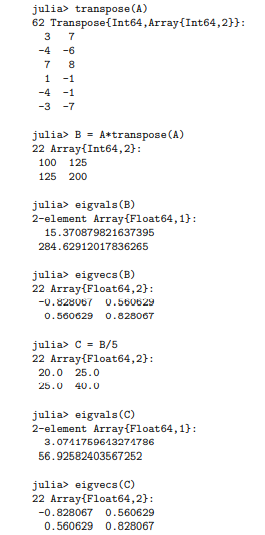
\includegraphics[width=6cm]{(19).png}
\end{center}



\end{document}
